
\section{802.15.4}

Defines \textbf{physical} and \textbf{MAC} layer for wireless Personal Area
networks (PAN). 2.4GHz, low range (75m), low rate (250kbits/s) for
low-power devices.

\textbf{Physical layer}: one form of CDMA

\subsection{Network topology}
Two types of nodes:
\begin{itemize}
    \item Full Functional Devices (FFD): can act as PAN coordinators
    \item Reduced Functional Devices (RFD): simple \& cheep
\end{itemize}
\begin{center}
    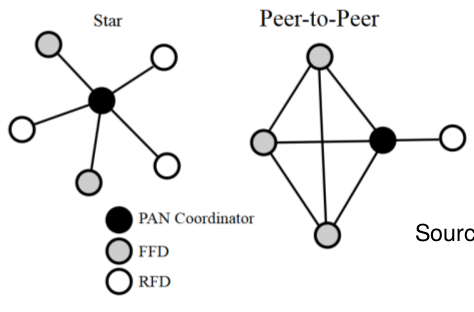
\includegraphics[width=0.5\linewidth]{img/802_topo.png}
\end{center}
Many upper-layer protocols define their own topologies
on top of the P2P topology.

\subsection{Addresses}
64-bits unique MAC address or 16 bits short address.
\begin{itemize}
    \item Too save memory: node get 16-bits short address
        assigned by coordinator when joining network (only
        valid inside PAN)
    \item Inter-PAN communication possible with a
        optional 16-bits PAN identifier
\end{itemize}

\subsection{Security}
Optional frame encryption supported with various
ciphers (e.g. AES-CCM 128 bit).
\begin{itemize}
    \item Frame header is authenticated, payload is encrypted
    \item Key management must be provided by higher layers
\end{itemize}

\subsection{Medium Access Control}
Implemented in software (as no need to very high performance):
\begin{itemize}
    \item CSMA/CA: wait idle channel or wait random backoff interval
        (0-2.24ms)
    \item Receiver check packet's CRC
    \item MAC layer can send ACK frame which are broadcasted
        (optional as many upper-layer protocols implements their
        own ACK mechanism)
\end{itemize}

\subsubsection{Unslotted mode}
Only CSMA/CA is used:
\begin{itemize}
    \item Very simple to implement 
    \item PAN coordinator not involved
    \item[But] need to continuously listen instead of sleep
        (power consuming)
\end{itemize}

\subsubsection{Slotted mode}

\begin{center}
    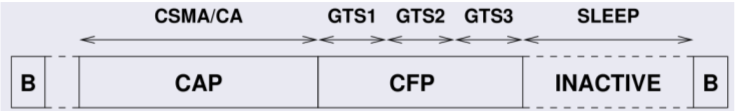
\includegraphics[width=0.5\linewidth]{img/slotted.png}
\end{center}

\begin{itemize}
    \item B = Beacon frame periodically sent by coordinator
    \item CAP = CSMA/CA period
    \item CFP = Guaranteed timeslots assigned by coordinator to nodes
    \item[Properties] 
        \begin{itemize}
            \item More complex. Requires coordinator.
            \item Allows Real-Time operation
            \item Nodes can sleep during inactivity period
        \end{itemize}
\end{itemize}

\section{Above 802.15.4}

\subsection{ZigBee}

Define on top of 802.15.4:
\begin{itemize}
    \item \textbf{Network layer}: 
        \begin{itemize}
            \item support slotted and unslotted mode,
                16-bits short addresses and 64-bits extended addresses
            \item Routing based on distance vector algorithm for tree, star
                and mesh topologies
        \end{itemize}
    \item \textbf{Security layer}: 128-bits AES, device responsible for
        key distribution
    \item \textbf{Application layer}: 
        \begin{itemize}
            \item High-level application framework that structure
                the capabilities of sensors in Application Objects
            \item Also provides service discovery, defines application
                profiles, message formats,...
        \end{itemize}
\end{itemize}

\subsection{Refresh IPv6}

\begin{center}
    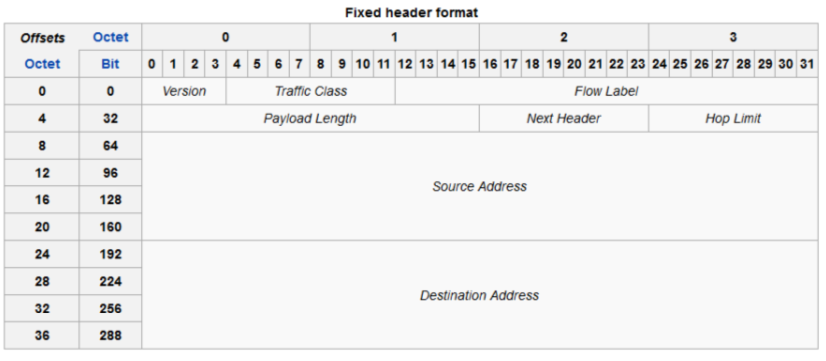
\includegraphics[width=0.7\linewidth]{img/IPV6.png}
\end{center}

\begin{itemize}
    \item \textbf{Addressing}
        \begin{itemize}
            \item Unicast: 128bits
                \begin{itemize}
                    \item 64bits for routing prefix and subnet id
                    \item 64bits for interface identifier
                    \item Global= 2000::...., 3FFF::....
                    \item Link local= FE80:0:0:0:....
                \end{itemize}
            \item Multicast: FF..::....
        \end{itemize}
    \item IPv6 Neighbor Discovery relies on multicast messages to:
        \begin{itemize}
            \item Router discovery (find router forwarding packets)
            \item Prefix discovery (find addresses using the prefix)
            \item Address resolution (replacing ARP for IPv4)
            \item Duplicate address detection
            \item Parameter discovery (MTU,...)
        \end{itemize}
\end{itemize}

\subsection{6LoWPAN}
IPv6 on 802.15.4:
\begin{itemize}
    \item IPv6 Header Compression (HC1): leave out unnecessary IPv6 header fields
    \item Fragmentation: because minimum IPv6 MTU = 1280 and Maximum
        frame size = 127bytes
    \item Link layer forwarding in mesh networks
\end{itemize}


\subsubsection{Stacked Header}
\begin{center}
    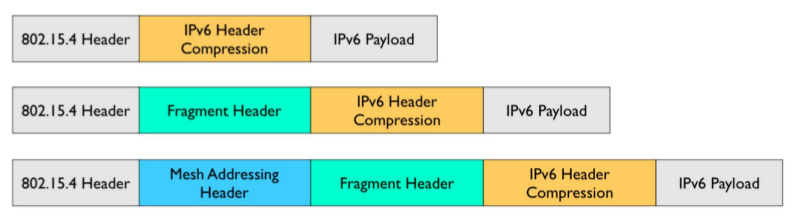
\includegraphics[width=0.7\linewidth]{img/stacked.png}
\end{center}

First byte (\textit{dispatch byte}) defines header type:
\begin{tabular}{rcl}
    00xxxxxx&:& not a 6LoWPAN frame\\
    01xxxxxx&:& IPv6 header (source/destination addr., etc.)\\
    10xxxxxx&:& Mesh header (for multi-hop forwarding)\\
    11xxxxxx&:& Fragment header (if packet is fragmented)\\
\end{tabular}

\paragraph{}

First byte for IPv6 header define IPv6 type: 
\begin{tabular}{rcl}
    01000001&:& uncompressed IPv6 header follows\\
    01000010&:& HC1-compressed IPv6 header follows (RFC 4944)\\
    011xxxxx&:& LOWPAN\_IPHC (RFC 6282)\\
\end{tabular}


\subsubsection{HC1}
\begin{itemize}
    \item \textbf{HC1 Header}: Ideally \begin{tabular}{l}
            First 64bits of IPv6 = link-layer address of 802.15.4 network\\
            Last 64bits of IPv6 = link-layer address (MAC)
        \end{tabular}

        $\Rightarrow$ No need to repeat them again in the HC1
        Header.

        \begin{center}
            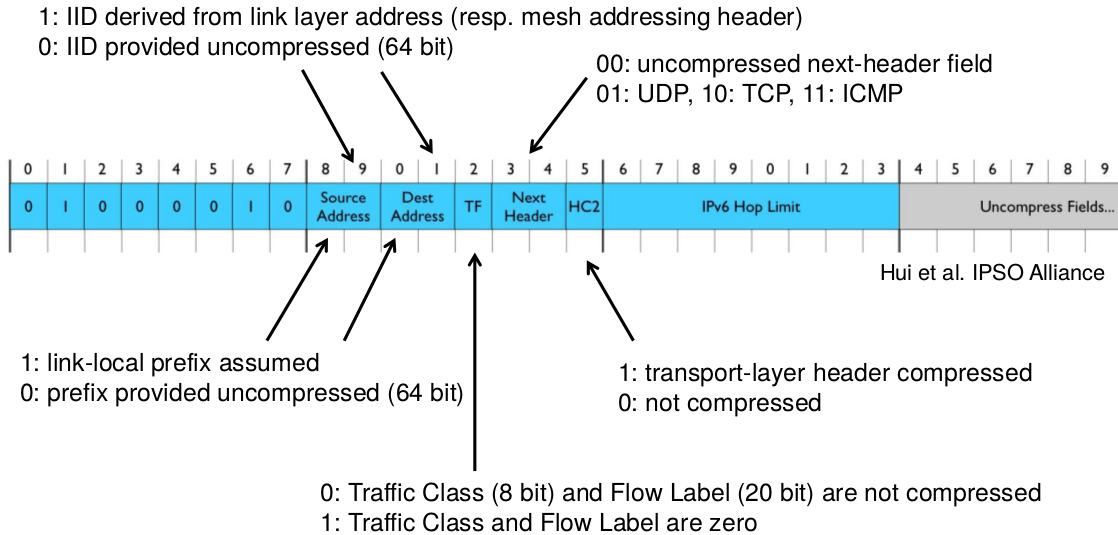
\includegraphics[width=0.9\linewidth]{img/HC1.png}
        \end{center}

    \item UDP Header Compression: If HC2 bit is set, a HC2 byte
        immediately follows the HC1 byte (before the hop-limit field)
        \begin{center}
            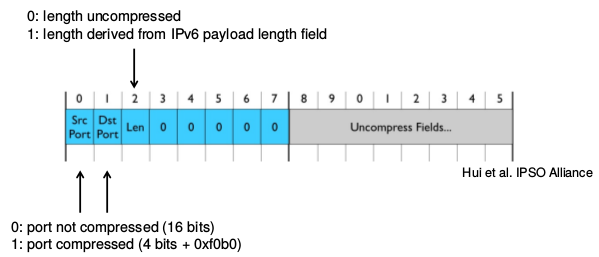
\includegraphics[width=0.7\linewidth]{img/UDP.png}
        \end{center}

        2bytes are also append for UDP checksum

        \proitem{} HC1+HC2 compression reduce UPD+IPv6 header to
        7bytes in the best case (link-local unicast addresses already
        contained in 802.15.4 frame)

        \consitem{} Advantage is lost if the 6LoWPAN device has to
        communicate with devices external to the 6LoWPAN $\Rightarrow$
        Routable addresses needed

        \begin{itemize}
            \item Full prefix has to be specified (64bit)
            \item Full IID has to be specified (64bit)
            \item Same for multi cast to IPv6 addresse
        \end{itemize}

\end{itemize}


\subsubsection{LOWPAN\_IPHC compression}
Replace HC1 Header

\begin{enumerate}
    \item[0-2]: define bits
    \item[3-4]: Traffic class and flow label 
    \item[5]: Next Header (0 uncompressed=8bit, 1: NH compressed
        with LOWPAN\_NHC)
    \item[6-7]: Hop-limit
\end{enumerate}

\paragraph{Addresses compression}
\begin{itemize}
    \item Stateless: Using the link-layer header fields (802.15.4) as HC1
    \item Stateful: share context information between nodes

        \textit{Context}: address prefix of length 0 to
        128bits, refers to remote or local addresses, specific lifetime

        \begin{itemize}
            \item Can specify a context in LOWPAN\_IPHC
            \proitem{} Can compress frequently used address prefixes
            \consitem{} Nodes have to store the context definitions
        \end{itemize}
\end{itemize}

\paragraph{Mesh addressing header}
IEEE 802.15.4 frames can only be sent single hop

\begin{itemize}
    \item If multi-hop mesh delivery is needed:
        \begin{itemize}
            \item RFDs discover FDDs and send all their traffic to them
            \item  FDDs do forwarding and run a routing protocol to populate their routing tables
        \end{itemize}
    \item With multi-hop, a packet has to carry two addresses:
        \begin{itemize}
            \item The link address of the next hop
            \item The link address of the original source and destination
            \item[$\Rightarrow$ ] Because the compressed IP header refers to it
        \end{itemize}
\end{itemize}

\begin{enumerate}
    \item 802.15.4 frame: specifies link-layer address of next hop
    \item  Mesh Addressing Header specifies original/final link-layer address
\end{enumerate}


